\section{Radno okruženje}
Za implementaciju rada izabran je Python programski jezik, koji je u posljednih godina dosegnuo visoku popularnost i koristi se u gotovo svim vrstama aplikacija. Interpretirani je jezik visoke razine opće namjene te ima filozofiju dizajna koji naglašava čitljivost k\^oda. Podržava više paradigme programiranja, uključujući objektno orijentirane, imperativne, funkcionalne i proceduralne. Programski jezik se dinamičko kuca (eng. \textit{dynamically typed}), što znači da varijablama se ne određuje tip, ali ako se želi postoji mogućnost izričito ga naglasiti. Posjeduje sveobuhvatnu biblioteku, koja između ostaloga pokriva i područje umjetne inteligencije. Korištenjem se dosta olakšavaju obrade i pripreme podataka za inteligentne agente, te izradu istih. Također, kako se nebi sukobili pakete iz ovog projekta sa paketima iz drugog ili iz sustava, stvorilo se posebno virtualno okruženje samo za ovaj projekt. Pythonov modul koji to omogućuje zove se \emph{virtualenv}.

\subsection{Integrirano razvojno okruženje}
K\^od je pisan u razvojnom okruženju PyCharm koji je jedan od mnogih okruženja Češke tvrtke JetBrains. Glavne značajke su analiza k\^oda, grafički program za otklanjanje pogrešaka, integrirani tester jedininca te integracija s kontrolnim sustavom za verzioniranje. Izgled PyCharm integriranog razvojnog okruženja prikazan je na slici~\ref{fig:pycharm}.
\\[\intextsep]
\begin{minipage}{\linewidth}
	\centering%
	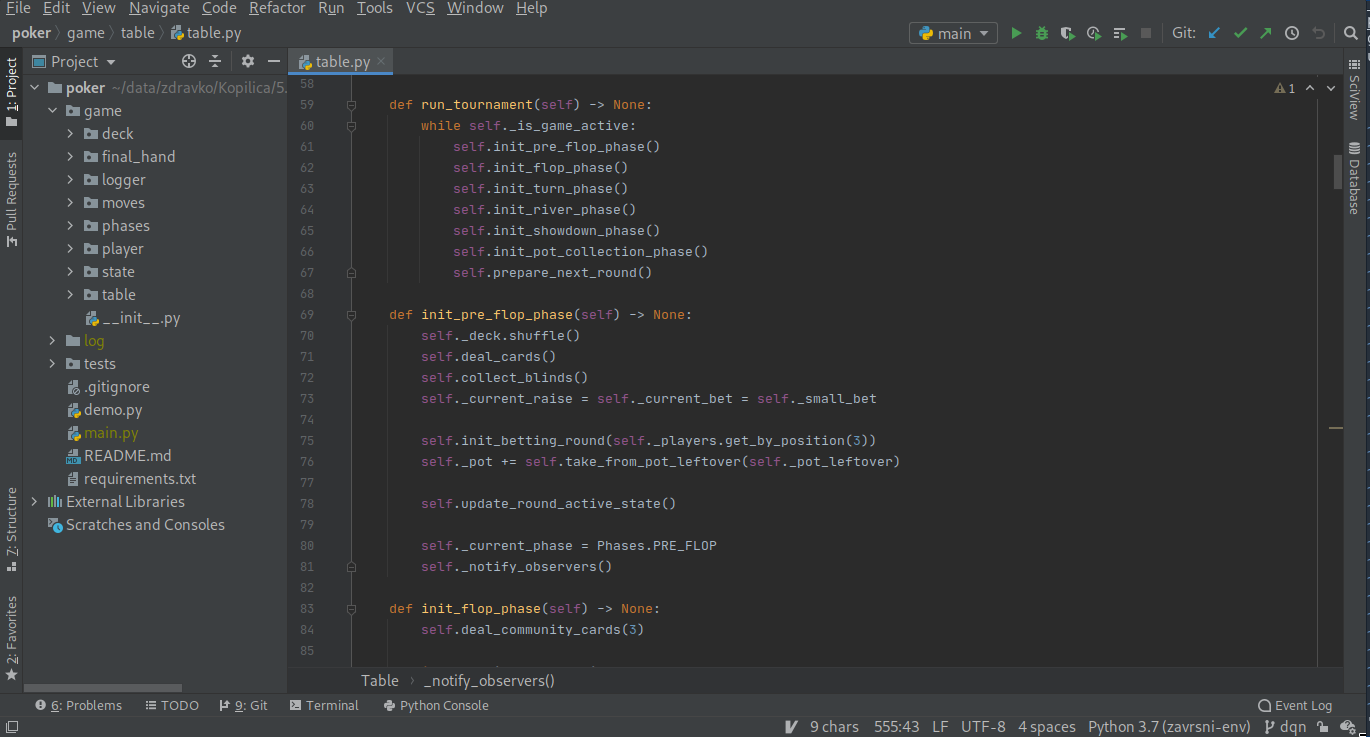
\includegraphics[width=0.8\linewidth,clip=]{images/pycharm.png}%
	\figcaption{Integrirano razvojno okruženje PyCharm}%
	\label{fig:pycharm}%
\end{minipage}
\\[\intextsep]

\subsection{Sustav za upravljanje verzijama}
Za praćenje promjene u izvornom k\^odu, korišten je git. Slobodan je i otvorenog k\^oda. Prilagođen je za rad programera, bilo to radu li više ljudi na istom projektu ili samo jedan. Stim da nije nužno da ga se koristi samo za praćenje promjene u izvornom k\^odu, nego za bilo koju vrstu datoteka. Osnovne značajke su mu brzina, integracija podataka, te podrška za distribuirane, ne linearne tijekovi rada. Također su se koristile poslužiteljske usluge GitHuba, na kojemu se nalazi izvorni k\^od ovoga rada. Putanja za pristup k\^odu je \url{https://github.com/zb46392/poker}. Github drži najveću količinu izvornog k\^oda na svijetu, te osim osnovnih funkcionalnosti gita, pruža dodatne usluge za upravljanje izvornim k\^odom. Među dodatnim značajkama se broje kontrola pristupa i prava, kolaboracijske alate za praćenje pogrešaka (eng. \textit{bug tracking}), upravljanje zadataka, pisanje dokumentacije itd.